\section{Experimental Setup}
    \subsection{Environment}
        We use the Farama Gymnasium's Ant-v4 environment \cite{Gymnasium2023} to evolve generalist MC-pairs. This environment consists of a flat plane for the ant to walk on with the objective to traverse a long distance. The ant's morphology comprises of four legs, each composed of an upper and a lower leg, with the upper leg attached to the torso. Figure~\ref{fig:ant_env} shows how the ant looks like. 
        \begin{figure}[ht]
            \centering
            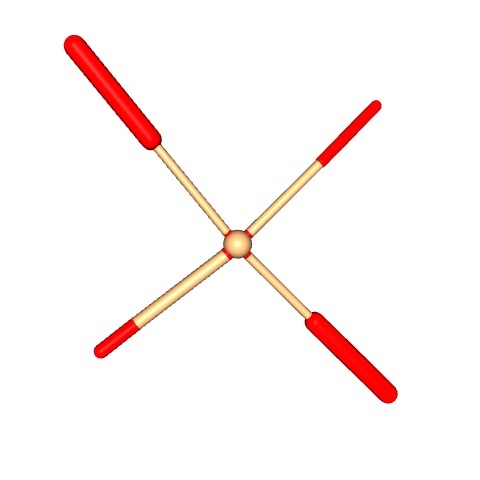
\includegraphics[width=0.9\linewidth]{./resources/ant_307.png}
            \caption{Example of an ant in the environment. The red legs depict the lower leg part and the light beige the upper leg part.}
            \label{fig:ant_env}
        \end{figure}
        To evolve a generalist MC-pair, we have to enable the ant to modify its morphology. Each leg part is parameterized into two atttributes: length and width, resulting in a total of 16 distinct morphological parameters. The leg lengths are constrained between 0.1 and 1.5, while the widths are limited from 0.08 to 0.2. 
        
        To ensure a fast and succesfull experiment, it was necessary to implement additional modifications to the ant's environment. We set the \seqsplit{$terminate\_when\_unhealthy$} flag to false, because it would terminate the run when the ant's torso of the ant ascends to a specific height. Disabling this allowed for the ant to become larger due to its capability to grow long leg lengths. Furthermore, we introduced additional settings to terminate the run whenever no significant movement forward was detected, suggesting that the ant froze into place. Another custom rule was implemented to detect if the ant flipped upsidedown by monitoring its z-vector. These two additional implementations reduced evaluation times significantly lower, especially at the start of the evolutionary process. 

    \subsection{Experimental parameters}
        For the controller, a fully connected feedforward ANN is evolved, based on the topology used by Triebold et al. \cite{Corinna_Triebold}, which consists of a single hidden layer with 20 neurons. The input layer corresponds to the ant's continuous observation space, which includes observations such as the angles between the torso and leg connections or velocity values, being in total 27 observations and thus 27 input nodes. The output layer corresponds to the ant's action space, where actions are values ranging from [-1, 1], representing the torque applied to the rotors, totaling 8 actions and thus 8 output nodes. Each layer also includes a bias node.
        
        For the parameters used in the XNES algorithm we used the default settings provided by the algorithm. The initial standard deviation of the search was set to 0.01 and the initial parameter ranges for the controller and encoded morphology parameters where [-0.1, 0.1]. To decode the morphology parameters a linear transformation is used where the lower bound morphology constraint maps to -0.1 and the upper bound morphology constraint maps to 0.1. The lower and upper bound constraints used for the length and width of the legs are [0.1, 1.5] [0.05, 0.2] respectively. \textbf{Should I also insert these linear transformation formula's that I used specifically?}
        
        The parameters used for the penalty function where decided based on initial experimental analysis we executed. For the growth rate $r^i$ we settled on 1.03 in conjunction with two scale factors for $\alpha$. This means we are using two different penalty functions. The reason being is that when the morphological parameters are decoded into negative values, the environment will crash due to not being able to have negative values for morphology. In these cases, $\alpha$ is set to 1000 and otherwise to 100.
        
        For the evolutionary process, we decided to evaluate the generalist scores after 2500 generation, instead of for every generation from the start. The reason being, to decrease the computational cost, but also because at the start of the evolutionary process, it is hard to gain high fitness scores, due to the search for a morphology to exploit effectively. After 2500 generations, a generalist score will be computed from the most fit individual in each generation. If after 200 generation no improvement is found, the process is terminated or a partition will occur.
    \subsection{Training data}
        The MC-pairs are training consist of different simulated environments, where the terrain is algorithmically generated based on the inputs. In this experiment, we consider three different environments. The first environment, referred to as the default environment, is a single static environment where the surface is flat. The two remaining environments are dynamically generated, named the rough terrain environment and the hill terrain environment. 
    \subsection{Testing and evaluation}